\documentclass{beamer}
\beamertemplatenavigationsymbolsempty

\title{Why is the Web Loosely Coupled?}
\author{Dustin Ingram}
\institute{Advances in Software Design, Spring 12-13\\ Drexel University
Department of Computer Science}
\date{\today}

\begin{document}
\maketitle

\begin{frame}
    \frametitle{The paper}
    \textbf{Why is the Web Loosely Coupled?}\\
    \textbf{A Multi-Faceted Metric for Service Design}\\
    \emph{C.~Pautasso (University of Lugano) \& E.~Wilde (UC Berkeley)}\\
    \begin{itemize}
        \item{Published 2009}
        \item{Proceedings of the 18th World Wide Web Conference}
    \end{itemize}
\end{frame}

\begin{frame}
    \frametitle{The problem}
    \begin{itemize}
        \item{``Coupling'' is a dichotomy;}
        \item{``Loosely coupled'' is essentially a buzz-word;}
        \item{No real metric for evaluating or comparing SOAs.}
    \end{itemize}
\end{frame}

\begin{frame}
    \frametitle{Goals of the paper}
    \begin{itemize}
        \item{More precisely define what `loose' and `tight' coupling means;}
        \item{Create a multi-faceted, non-dichotomous metric for coupling;}
        \item{Systematic study of degree of coupling in three popular SOAs;}
    \end{itemize}
\end{frame}

\begin{frame}
    \frametitle{What do we think ``loosely coupled'' means?}
    \begin{quote}
        ``The notion of designing services to be loosely coupled is the most important,  the most far  reaching, and the least understood service characteristic.''
    \end{quote}
    \hfill ---E. Newcomer \& G. Lomow,\\\hfill \emph{Understanding SOA with Web services}

\end{frame}

\begin{frame}
    \frametitle{What do we think ``loosely coupled'' means?}
    A general positive connotation:
    \begin{itemize}
        \item{Small set of assumptions;}
        \item{Impact of change is limited;}
        \item{Easy and cheap to evolve;}
        \item{Potential to scale.}
    \end{itemize}
\end{frame}

\begin{frame}
    \frametitle{What do we think ``loosely coupled'' means?}
    The alternative:
    \begin{itemize}
        \item{Huge set of assumptions;}
        \item{Impact of change is immense;}
        \item{Hard and expensive to evolve;}
        \item{Can't scale.}
    \end{itemize}
\end{frame}

\begin{frame}
    \frametitle{Why \emph{is} the web loosely coupled?}
    \begin{quote}
        ``Decentralization is another important design feature. You do not have to get approval from any central authority to add a page or make a link... Decentralization has made widespread innovation possible and will continue to do so in the future.''
    \end{quote}
    \hfill ---Tim Berners-Lee\footnote{\scriptsize{\url{http://www.scientificamerican.com/article.cfm?id=long-live-the-web}}}
\end{frame}

\begin{frame}
    \frametitle{Why \emph{is} the web loosely coupled?}
    \begin{itemize}
        \item By design;
        \item By evolution.
    \end{itemize}
\end{frame}

\begin{frame}
    \frametitle{What is a SOA?}
    A software design methodology, advocating:
    \begin{itemize}
        \item Delineation between Client and Server models;
        \item Discretization of individual service components;
        \item Reuse through reorganization;
        \item Common protocol for interoperation (XML, JSON);
        \item Loose coupling!
    \end{itemize}
\end{frame}

\begin{frame}
    \frametitle{The architectures}
    Three service-oriented architectures:
    \begin{itemize}
        \item{RESTful HTTP}
        \item{RPC over HTTP}
        \item{WS-*/ESB}
    \end{itemize}
\end{frame}

\begin{frame}
    \frametitle{RESTful HTTP}
    Representational State Transfer over HTTP:
    \begin{itemize}
        \item Introduced and defined by Roy Fielding in 2000;
        \item Key concepts:
        \begin{itemize}
            \item Re-use of HTTP verbs (e.g., \texttt{GET}, \texttt{PUT}, etc.);
            \item Exchange of resource representation;
            \item Full asynchrony and statelessness.
        \end{itemize}
        \item Often conflated with RESTful API design.
        \item Not a standard!
    \end{itemize}
\end{frame}

\begin{frame}
    \frametitle{RPC over HTTP}
    Remote Procedure Call over HTTP:
    \begin{itemize}
        \item Introduced by Bruce Jay Nelson at Xerox PARC in the 1980's
        \item Key concepts:
        \begin{itemize}
            \item Synchronous, blocking request from client to server;
            \item Essentially a function call (function name, parameters).
        \end{itemize}
        \item There are a number of RPC standards.
    \end{itemize}
\end{frame}

\begin{frame}
    \frametitle{WS-*/ESB}
    WS-* is a large collection of web service standards:
    \begin{itemize}
        \item No single creator, nor ``official'' set;
        \item Standards may complement and/or compete.
    \end{itemize}
    Enterprise Service Bus
    \begin{itemize}
        \item Focus on explicit management of inter-service messaging;
        \item No official standard.
    \end{itemize}
\end{frame}

\begin{frame}
    \frametitle{Evaluating the coupling of SOAs}
    The components of the coupling of a SOA are complex:
    \begin{itemize}
        \item Consist of multiple ``facets'';
        \item Facets are not necessarily orthogonal;
        \item Facets do cover all relevant design aspects.
    \end{itemize}
\end{frame}

\begin{frame}
    \frametitle{The facets}
    \begin{columns}[T]
      \begin{column}{.5\linewidth}
        \begin{enumerate}
            \item{Discovery}
            \item{Identification}
            \item{Binding}
            \item{Platform}
            \item{Interaction}
            \item{Interface Orientation}
        \end{enumerate}
      \end{column}
      \begin{column}{.5\linewidth}
        \begin{enumerate}
          \setcounter{enumi}{6}
            \item{Model}
            \item{Granularity}
            \item{State}
            \item{Evolution}
            \item{Generated Code}
            \item{Conversation}
        \end{enumerate}
      \end{column}
   \end{columns}
\end{frame}

\begin{frame}
    \frametitle{Visualizing coupling facets}
    \begin{figure}
        \centering
        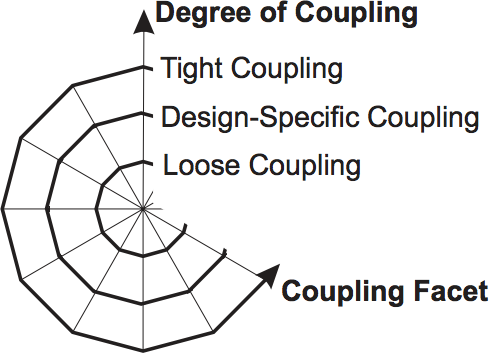
\includegraphics[height=0.6\paperheight]{fig3-0.png}
    \end{figure}
\end{frame}

\begin{frame}
    \frametitle{Facet \#1: Discovery}
    \begin{itemize}
        \item Compulsory registration of services, or lack thereof;
        \item Example: DNS on the web;
        \item Example: Open Directory Project vs. Search Engines;
        \item Tight coupling: explicit registration;
        \item Loose coupling: decentralized referral.
    \end{itemize}
\end{frame}

\begin{frame}
    \frametitle{Facet \#2: Identification}
    \begin{itemize}
        \item Essentially the naming of systems;
        \item Defining the association between the representations;
        \item Example: In RESTful architectures, using URI identification schemes;
        \item Tight coupling: context-based;
        \item Loose coupling: global.
    \end{itemize}
\end{frame}

\begin{frame}
    \frametitle{Facet \#3: Binding}
    \begin{itemize}
        \item Process of resolving symbolic names into low-level identifiers;
        \item Example: binding a DNS name to an IP address;
        \item Tight coupling: early;
        \item Loose coupling: late.
    \end{itemize}
\end{frame}

\begin{frame}
    \frametitle{Facet \#4: Platform}
    \begin{itemize}
        \item Concerns the requirements for services to be based on a homogeneous middleware infrastructure;
        \item Might require complex bridging solutions;
        \item With many platforms available, web protocol standards become important;
        \item Tight coupling: dependent;
        \item Loose coupling: independent.
    \end{itemize}
\end{frame}

\begin{frame}
    \frametitle{Facet \#5: Interaction}
    \begin{itemize}
        \item Answers the question, ``Do all services need to be available at the same time?''
        \item Example: vanilla HTTP vs. HTTP w/ caches, proxies and reverse proxies;
        \item Tight coupling: synchronous;
        \item Loose coupling: asynchronous.
    \end{itemize}
\end{frame}

\begin{frame}
    \frametitle{Facet \#6: Interface Orientation}
    \begin{itemize}
        \item Horizontal interfaces are local interfaces from a higher-level component to a lower-level component;
        \item Layered architectural style;
        \item Vertical interfaces have components on the same abstraction level;
        \item Do not make assumptions about the local abstraction;
        \item Tight coupling: horizontal;
        \item Loose coupling: vertical.
    \end{itemize}
\end{frame}

\begin{frame}
    \frametitle{Facet \#6: Interface Orientation}
    \begin{figure}
        \centering
        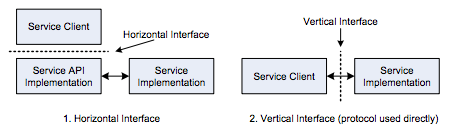
\includegraphics[width=0.8\paperwidth]{fig2.png}
    \end{figure}
\end{frame}

\begin{frame}
    \frametitle{Facet \#7: Model}
    \begin{itemize}
        \item Common application-level data model shared among services;
        \item Or, services share messages which have a standardized representation format;
        \item Tight coupling: shared model;
        \item Loose coupling: self-describing messages.
    \end{itemize}
\end{frame}

\begin{frame}
    \frametitle{Facet \#8: Granularity}
    \begin{itemize}
        \item Tradeoff between number of interactions to provide functionality and complexity of the data parameters.
        \item The fewer the interactions, the coarser the interface;
        \item Tight coupling: fine;
        \item Loose coupling: coarse.
    \end{itemize}
\end{frame}

\begin{frame}
    \frametitle{Facet \#9: State}
    \begin{itemize}
        \item State management cam become one of the central problems in efficient service design;
        \item Maintaining multiple instance of the representation of an interaction can be difficult;
        \item Both are necessary (e.g., sessions, cookies);
        \item Tight coupling: shared, stateful;
        \item Loose coupling: stateless.
    \end{itemize}
\end{frame}

\begin{frame}
    \frametitle{Facet \#10: Evolution}
    \begin{itemize}
        \item Change of a service over time, and how it affects the clients;
        \item Backward \& forward compatibility;
        \item Closely related to the discovery facet;
        \item Tight coupling: breaking, exact version matching;
        \item Loose coupling: multi-version compatibility.
    \end{itemize}
\end{frame}

\begin{frame}
    \frametitle{Facet \#11: Generated Code}
    \begin{itemize}
        \item Automatic generation of code to handle key communications functions;
        \item Needs requirements specified at runtime;
        \item Required dependency on runtime environment;
        \item Tight coupling: static;
        \item Loose coupling: none/dynamic.
    \end{itemize}
\end{frame}

\begin{frame}
    \frametitle{Facet \#12: Conversation}
    \begin{itemize}
        \item Service invocations span multiple basic interactions;
        \item Prescribed set of partially ordered message exchanges;
        \item Example: using hyperlinks to steer participating clients;
        \item Example: replying to a form submission with a new form;
        \item Tight coupling: explicit;
        \item Loose coupling: reflective.
    \end{itemize}
\end{frame}

\begin{frame}
    \frametitle{Evaluation}
    \begin{figure}
        \centering
        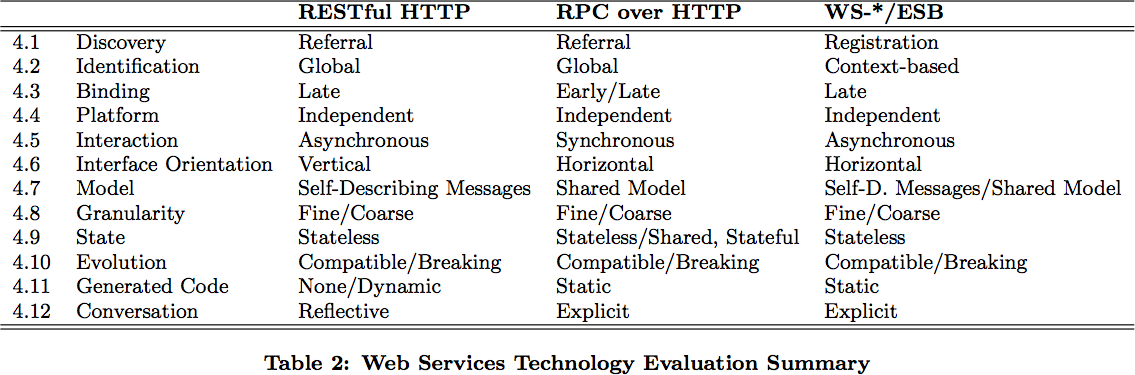
\includegraphics[width=0.8\paperwidth]{table2.png}
    \end{figure}
\end{frame}

\begin{frame}
    \frametitle{Visualizing coupling facets}
    \begin{figure}
        \centering
        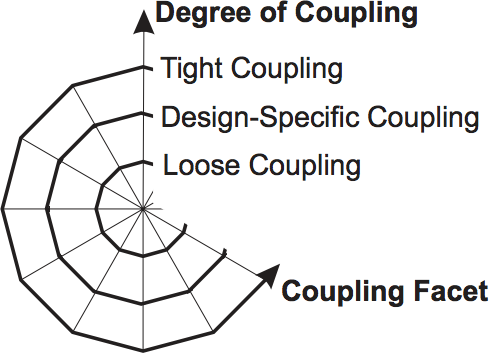
\includegraphics[height=0.6\paperheight]{fig3-0.png}
    \end{figure}
\end{frame}

\begin{frame}
    \frametitle{RESTful HTTP}
    \begin{figure}
        \centering
        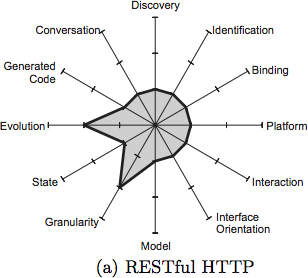
\includegraphics[height=0.6\paperheight]{fig3-1.png}
    \end{figure}
\end{frame}

\begin{frame}
    \frametitle{RPC over HTTP}
    \begin{figure}
        \centering
        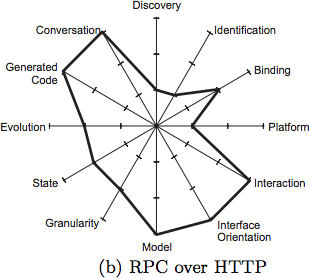
\includegraphics[height=0.6\paperheight]{fig3-2.png}
    \end{figure}
\end{frame}

\begin{frame}
    \frametitle{WS-*/ESB}
    \begin{figure}
        \centering
        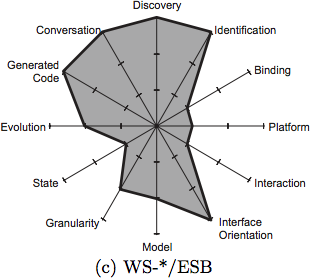
\includegraphics[height=0.6\paperheight]{fig3-3.png}
    \end{figure}
\end{frame}

\begin{frame}
    \frametitle{Conclusion}
    \begin{itemize}
        \item The twelve facets give a better metric for `coupled'-ness;
        \item Very few systems are truly entirely `tightly' or `loosely' coupled in all facets;
        \item Ultimately, allows one to make better comparisons and design decisions.
    \end{itemize}
\end{frame}
\end{document}
